In this section, we describe our general methodology for evaluating ML models to detect anomalies in cloud gaming sessions. We first formulate the anomaly detection task for anomalous windows in CG sessions and introduce the collected datasets. Our new approach, called Window Anomaly Decision (WAD), proposed to address the limitations of existing window approaches, is then presented. This is followed by an introduction on the unsupervised ML models used in our comparative evaluation.


\subsection{Problem statement}
Our goal in this paper is to detect the end-users' QoE degradation in CG sessions. For this, we decided to base our detection analysis using windows of observations, instead of individual points of observation. Indeed, QoE degradation lasting 5ms is not perceptible by human beings for whom the perception of latency is around 150ms \cite{Amano2006EstimationOT}. Therefore, we evaluate the ML models with 3 window sizes $p \in \{10,20,30\}$ to perform a detection within $50, 100, 150$ ms respectively, and have a representative time of perception (i.e., very reactive people to less reactive ones, via mean value).

As such, we can formalize our problem as follows: we denote the time-series of our datasets as $x = \{x_1,x_2, ..., x_T\}$, where $T$ is the length of $x$ and $x_t \in \mathbb{R}^m$ denotes a $m$-dimensional vector corresponding to the values of our $m$ features at time $t$. For the representation of observations in windows, we split $x$ into sequences of windows $W = \{w_1, w_2, ..., w_{T-p+1}\}$ with stride 1 where $w_t = \{x_t, x_{t+1}, ..., x_{t+p-1}\}$, $p$ being the window size.

Given an unsupervised anomaly detection model $\mathcal{M}$, a set of parameters $\mathcal{W}$ is learnt to output an anomaly score $s(\tilde{x_t})$ for each unseen observation $\tilde{x_t}$. From this anomaly score and a carefully chosen threshold $\delta$, a binary variable $\tilde{y_t} \in \{0,1\}$ is assigned for each observation as follows:
\begin{equation}
    \tilde{y_t} = 
    \begin{cases}
       1, & \text{if } s(\tilde{x_t}) > \delta \\
       0, & \text{otherwise.}
    \end{cases}
\end{equation}

The goal of the window-based detection of anomalies is to correctly map the binary value of each observation within a window to a binary value for the whole window. Since we focus on perceptible end-users’s QoE degradation, a large part of the window observations should be anomalous so that the windows is classified as anomalous. In the remainder of the paper, we consider a window as anomalous if at least 80\% of observations in the window are anomalous.

% Include a tab of features
\begin{table}[t]
\begin{threeparttable}
\caption{Description of collected features}
\label{tab:chap_3:datasets_description}
\setlength\tabcolsep{1pt} % make LaTeX figure out intercolumn spacing

\begin{tabular*}{\hsize}{@{\extracolsep{\fill}} l l}
\toprule
       \bf Features  & \bf Description \\
\midrule
      \multirow{1}{*}{Network RTT} & Network RTT computed during game session. \\
      \addlinespace
     \multirow{1}{*}{Decoding delay} & Delay to decode each video frame. \\
     \addlinespace
     \multirow{3}{*}{Jitter buffer delay} & Delay between the time, the first packet of a \\
                                         & video frame enters the jitter buffer and the time \\
                                         & the whole frame exits the jitter buffer.\\
   \addlinespace
     \multirow{1}{*}{Video rendering jitter} & Time between two consecutive video frames.\\
      \addlinespace

% \addlinespace
% \midrule
     \multirow{1}{*}{Uplink Bitrate} &  Number of bits-per-second (bps) sent by the client.\\
      \addlinespace
      \multirow{1}{*}{Downlink Bitrate} &  Number of bits-per-second (bps) received by the client.\\
      \addlinespace
    \multirow{1}{*}{Frame rate} & Frames received per-second (FPS).\\
     \addlinespace
    \multirow{1}{*}{Height resolution} & Number of pixels in the frame height.\\
     \addlinespace
    \multirow{1}{*}{Width resolution} & Number of pixels in the frame width. \\
     \addlinespace
    \multirow{3}{*}{Freeze} & A freeze is count if an inter-frame delay is greater than   \\
    & a value defined as $max(3*avgInterFrameDelay,$\\
    &  $avgInterFrameDelay + 150ms)$. \\
     \addlinespace
    \multirow{2}{*}{Frames dropped} & Number of video frames dropped before \\
        & decoding step. \\
     \addlinespace
    \multirow{1}{*}{Frames decoded} & Number of video frames decoded.\\
     \addlinespace
    \multirow{1}{*}{Packets received} & Number of packets received.\\
     \addlinespace
% \addlinespace
% \midrule
\multirow{2}{*}{Downlink throughput}  & Max downlink capacity allowed by \\
                                        & the 4G network conditions.\\
                               

\addlinespace
\bottomrule
\end{tabular*}
\end{threeparttable}
\end{table}


\subsection{Data collection}
We rely on the datasets used in our previous work \cite{Ky2022}\footnote{Datasets are available as OpenData : \url{https://cloud-gaming-traces.lhs.loria.fr/ANR-19-CE25-0012_std_gfn_xc_cg_webrtc_metrics.7z}} which contain time-series features of QoE and QoS collected while playing racing games on public cloud gaming platforms:
\begin{itemize}
    \item \textit{Dirt 4} for Google Stadia (STD);
    \item \textit{TrackMania} for Nvidia GeForce Now (GFN);
    \item \textit{F1 2021} for Microsoft Xbox Cloud (XC).
\end{itemize}
A set of 14 features (cf. Table \ref{tab:chap_3:datasets_description}) were collected through the Chromium WebRTC API adapted by the DECAF tool \cite{Iqbal2021DissectingCG}. The measurements were performed under 6 different 4G network conditions, with 5 differing in the average downlink throughput and 1 in a mobility scenario on a highway. 
More details about the testbed, the network conditions and the datasets are available in \cite{Ky2022}.

The collected datasets are unlabelled (i.e., with no ground-truths). Consequently, evaluation of the models performance with well-known ML evaluation metrics, such as Precision, Recall or F1-score is not possible. We hence create ground-truth $(y_t)_{t\in \|1,T\|}$ (i.e., labels) for evaluation purposes (and intrinsically to split the data), but the labels are not used by ML algorithms during training. According to the CG platform's recommendations for high quality streaming,\footnote{\url{https://support.google.com/stadia/answer/9607891?hl=fr/}} \footnote{\url{https://www.nvidia.com/en-us/geforce/products/geforce-now/system-reqs/}} we define the ground-truths based on the following criteria ($\gamma = 1080$ for STD and XC and $\gamma = 768$ for GFN):

\begin{equation}
    y_t = 
    \begin{cases}
       1, & \text{if } \begin{cases}
                            resolution(x_t) <& \gamma \text{ or}  \\
                            frameRate(x_t)  <& 60 \text{ or} \\
                            freeze(x_t) =& 1 
                        \end{cases} \\
       0, & \text{otherwise.}
    \end{cases}
\end{equation}
\\


We would like to stress here that the primary objective of this paper is to compare the performance of unsupervised ML models in detecting anomalies on a CG case study. The objective is not to detect degradation using simple rules, but rather to utilize such rules to establish ground-truths required for computing the ML metrics. Although being simple, there rules present a significant challenge for our tasks, particularly when they are unknown a-priori as shown later in the paper our results in Section \ref{chap_3:evaluation}.

Using these ground-truth labels as a reference, we define a ground-truth window as anomalous if at least $80\%$ of the labels of the window are anomalous.

\subsection{Data processing and splitting}
The features of the datasets are resampled to have a fixed time-step of 5ms and they are normalized before training.
We build the training and testing sets following the splitting strategy proposed by Zong et al. \cite{zong2018deep} which ensures consistency over different experiments and allow to perform a fair evaluation. The entire dataset is split as follows: $50\%$ of the normal samples are associated to the training set while the remaining $50\%$ are considered as a test set. The test set also contains $60\%$ of the anomalous samples. The remaining $40\%$ of the anomalous samples compose a set called the contamination set. The anomalous samples in the latter set, are actual instances of anomalies that occurred during gameplay, and were subsequently collected in our datasets. They serve to \textit{contaminate} the training set with anomalous samples (with a ratio $c\in\{0\%,4\%,8\%,12\%,20\%\}$) and study the robustness of ML algorithms to data contamination. The rationale behind this splitting strategy is to maintain consistency across various experiments and ensure fairness in evaluating model performance under conditions of data contamination.
 Table \ref{tab:chap_3:datasets} shows the summary of our datasets after the splitting step.
 
 % Add tab for datasets stats
\begin{table}[t]
\begin{threeparttable}
\caption{Datasets summary}
\label{tab:chap_3:datasets}
\setlength\tabcolsep{0pt} % make LaTeX figure out intercolumn spacing

\begin{tabular*}{\columnwidth}{@{\extracolsep{\fill}} l c c c c}
\toprule
      \bf Datasets &  \bf Train normal  & \bf Contamination  &  \bf Test & \bf Test anomalies \\
      & \bf windows & \bf set windows & \bf windows & \bf ratio (\%) \\
\midrule
        \bf STD & 80486 & 59480 & 169706 & 52.57 \\
\addlinespace
        \bf GFN & 27415 & 22667 & 61417 & 55.36 \\
\addlinespace
        \bf XC & 83611 & 17918 & 110487 & 24.32 \\


\bottomrule
\end{tabular*}
\end{threeparttable}
\end{table}



\subsection{Existing window evaluation approaches}
As mentioned in Section \ref{window_metrics}, PW approaches are unsuitable for AD in CG sessions and window approaches are preferred. PA, PA$\%K$ and RPA approaches were proposed in \cite{xu2018unsupervised} \cite{Kim2022TowardsAR} and \cite{hundman2018detecting} respectively. 

PA approach assumes that if any observation in a ground-truth anomaly segment is correctly detected, all the observations in this segment are considered as anomalous and correctly detected (i.e., $p$ true positives are recorded). If none of the observations in the ground-truth anomaly segment is correctly detected, $p$ false negatives are recorded. Observations that are not in a ground-truth anomaly segment are treated as point-wise. 


RPA approach behaves in the same way as PA but for ground-truth anomaly segment: instead of recording $p$ true positives, it records only 1 true positive for the whole window if any observation in a ground-truth anomaly segment is correctly detected. It records 1 false negative if none of the observations in the ground-truth anomaly segment is correctly detected. The observations that are not in a ground-truth anomaly segment are treated as point-wise. 

PA$\%K$ approach aims to minimize overestimation errors in the PA approach by using a hyper-parameter $K$ to adjust the anomaly prediction threshold. Specifically, PA$\%K$ considers an anomaly segment to be correctly detected if at least $K\%$ of its observations are accurately detected (i.e. $p$ true positives are recorded if so and $p$ false negatives otherwise.). The observations outside of a ground-truth anomaly segment are treated as point-wise.


Analysing this behavior (and later demonstrated by our experiments in Section \ref{wad_metrics}), we can first observe that the PA approach is more tolerant to high false positive rates in a large anomaly windows and hence leads to high scores, thereby overestimating the performance of a model. In contrast, the RPA approach gives lower scores due to its differential and unfair evaluation between anomaly windows and normal windows. Classifying a window as anomalous, based on only one observation correctly detected (as done by PA/RPA approach) can result in many false alarms, which can have extra unnecessary costs and makes the detection model unpractical. Moreover, the three aforementioned approaches necessitate having access to accurate ground-truth segments in order to evaluate the model.

Given the limitations and shortcomings of these approaches when comparing various ML models, 
we therefore propose a Window Anomaly Decision (WAD) approach to accurately evaluate ML models for window-based anomaly detection. 

\begin{figure*}[!t]
  \centering
  \begin{tabular}{ c @{\hspace{0pt}} c}
  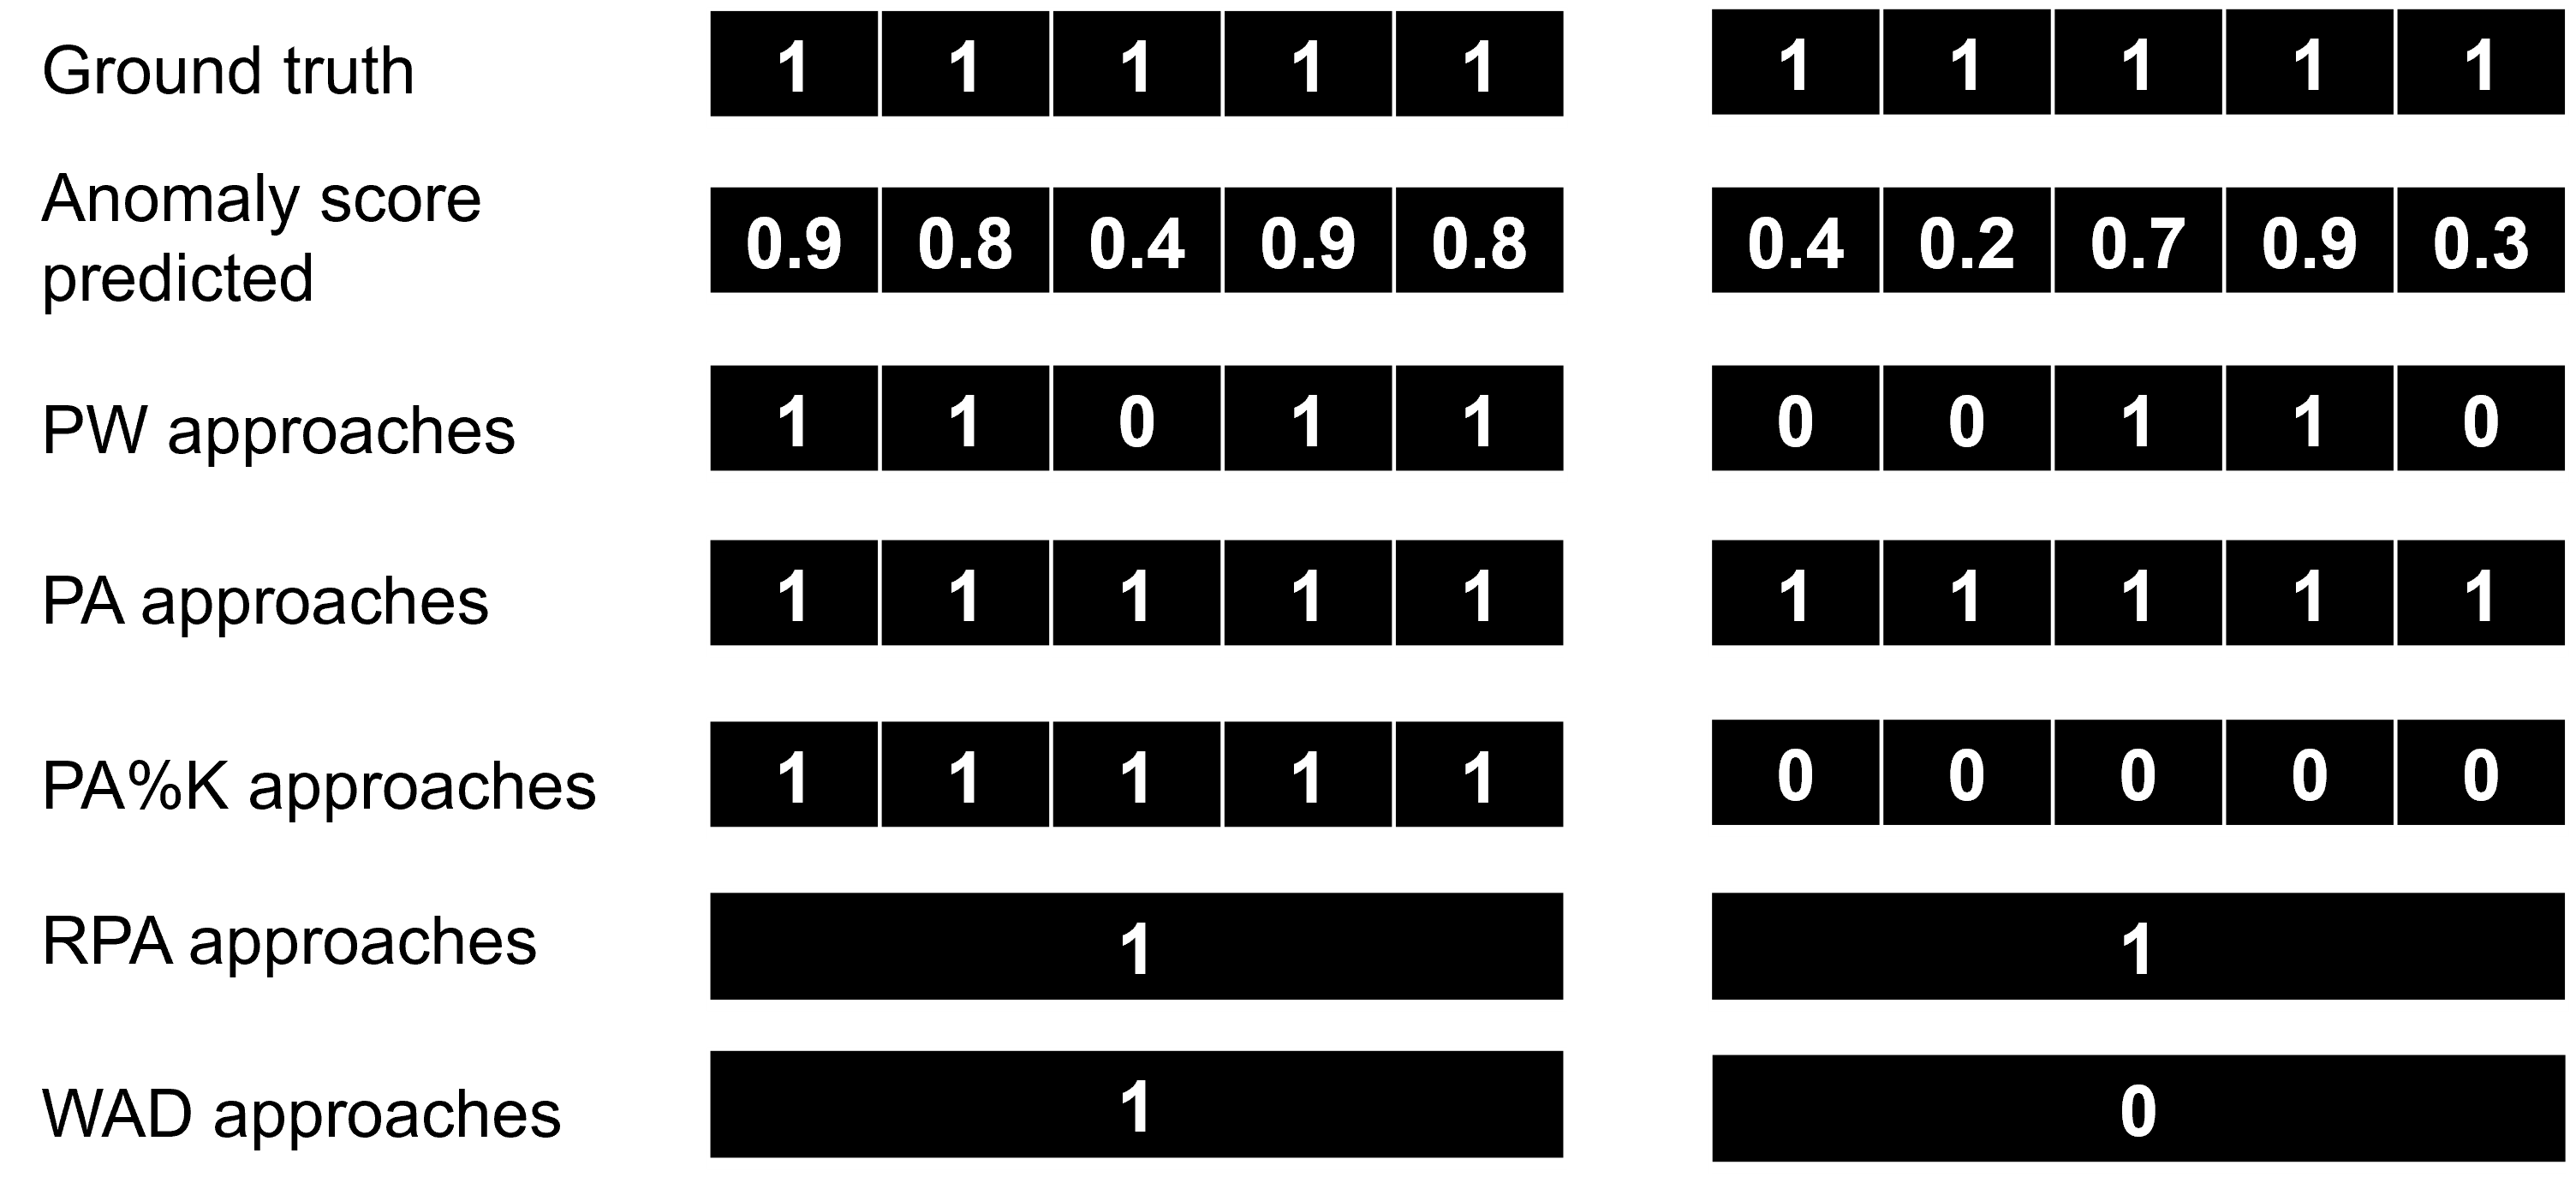
\includegraphics[width=0.5\textwidth]{imgs/chapter_3/window_comparison_1.png}
    &
  %\medskip
    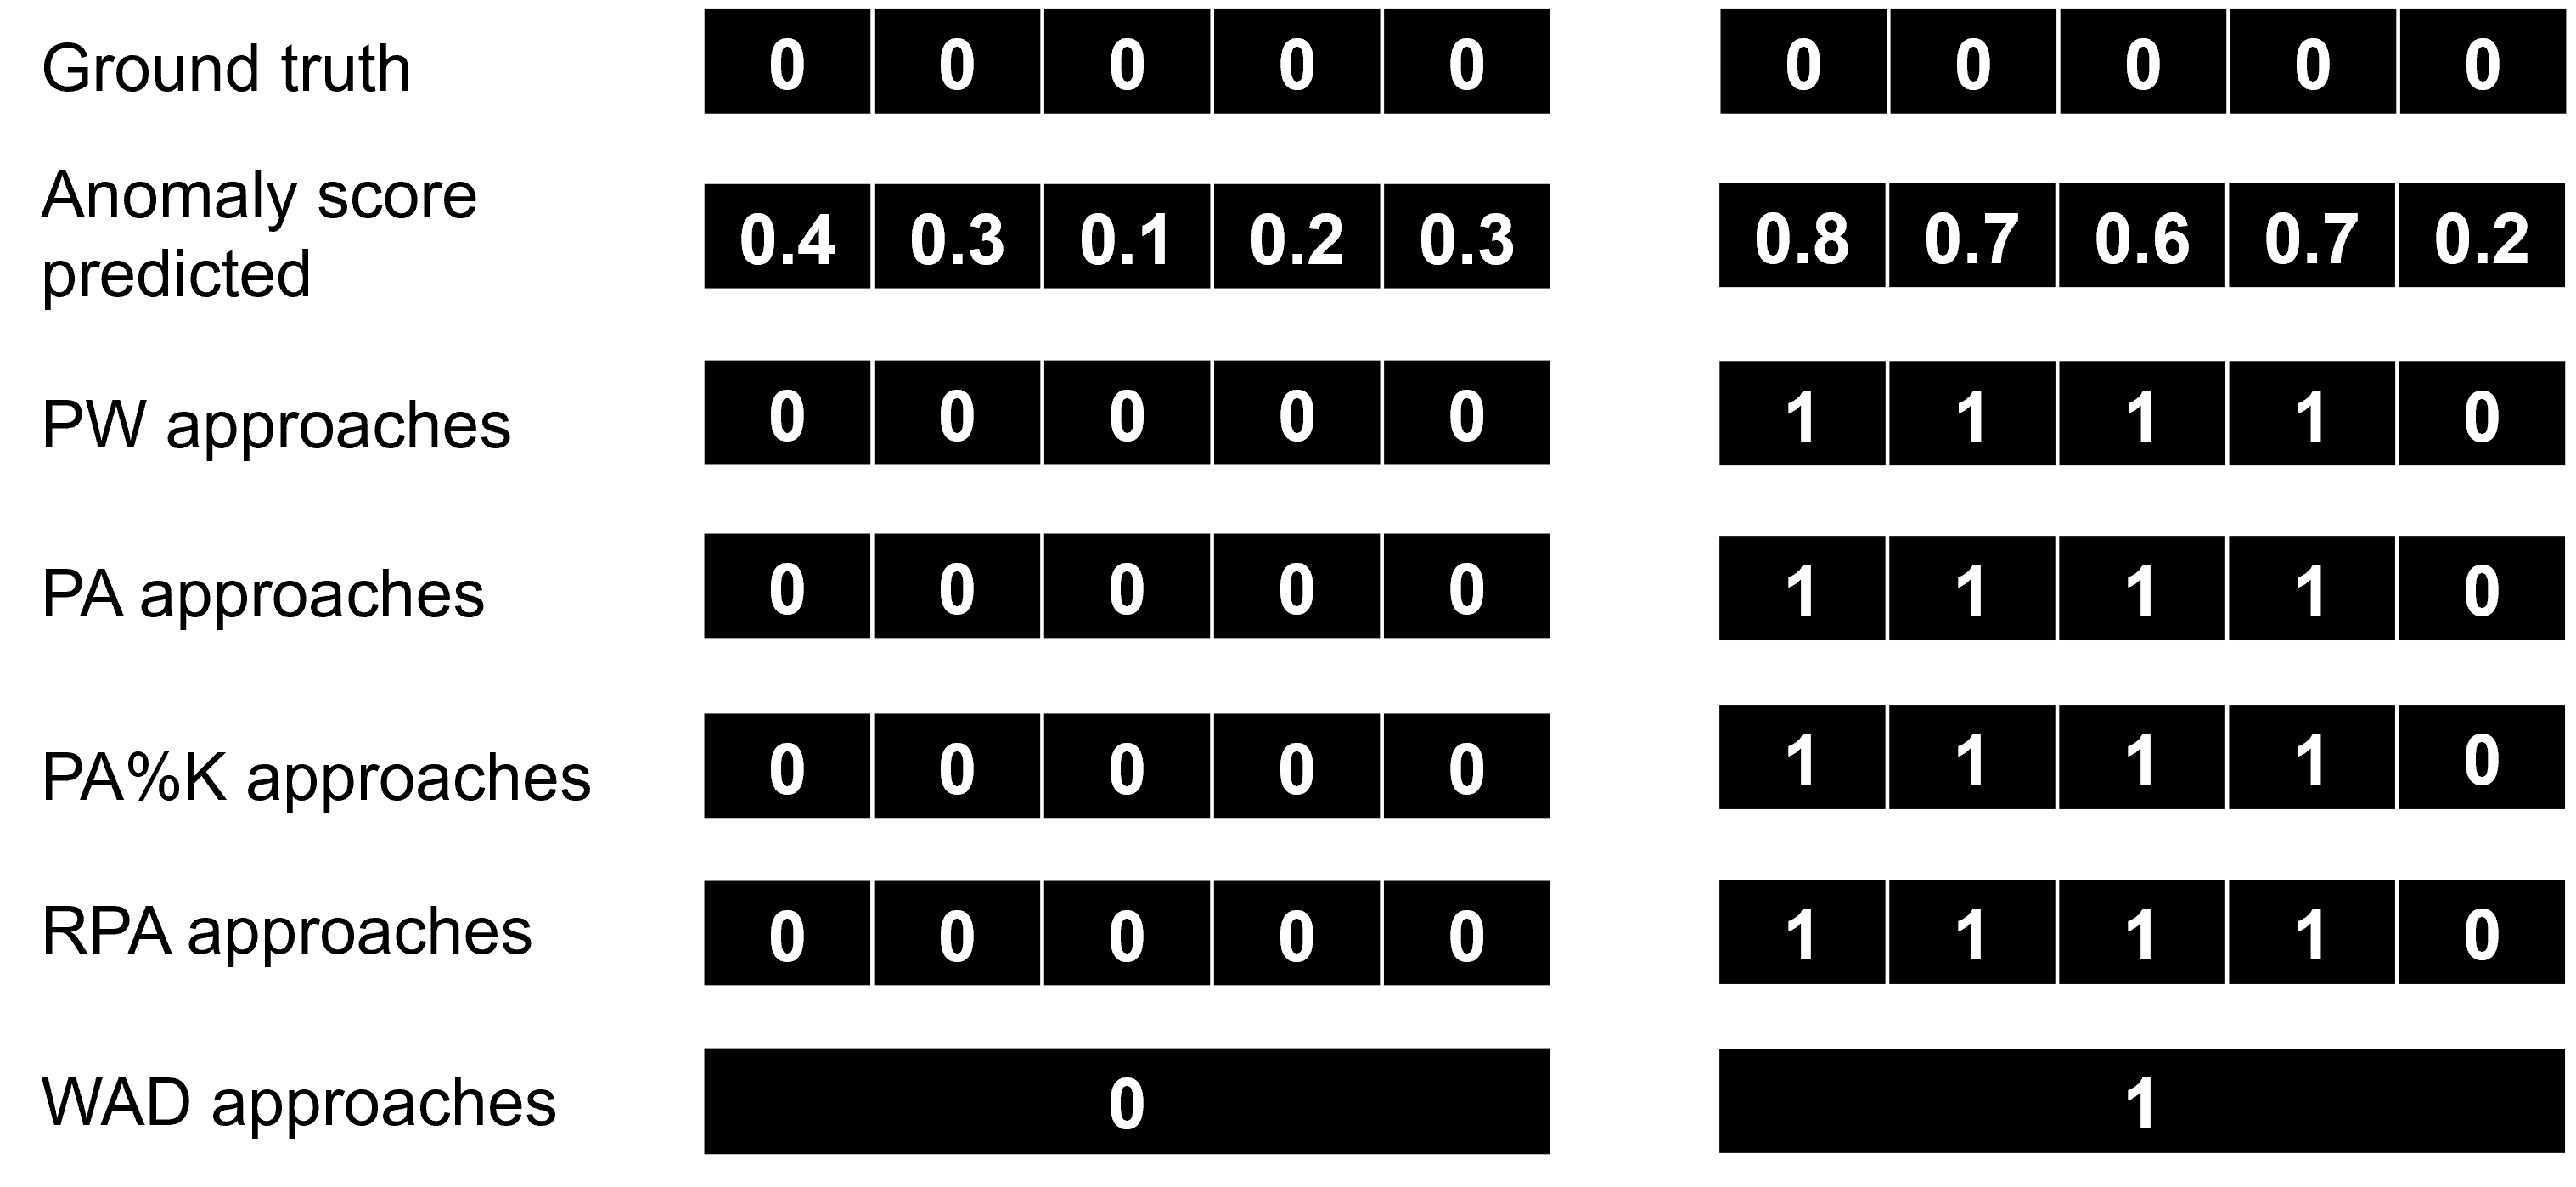
\includegraphics[width=0.5\textwidth]{imgs/chapter_3/window_comparison_2.png} \\
     \small \textbf{(a) Prediction on anomaly windows} &
    \small \textbf{(b) Prediction on normal windows}  \\
  \end{tabular}
  \medskip
  \caption{Illustration of PW, PA, RPA and WAD approaches. 0 is normal and is 1 anomalous. The anomaly score threshold to decide if an observation is anomalous or not is $\delta = 0.5$. Window size $p=5$, $\alpha = 0.8.$}
  \label{fig:chap_3:window_comparison}
\end{figure*}


\subsection{Window Anomaly Decision (WAD) approach}

WAD approach is designed to fairly evaluate anomalous and normal windows. Furthermore, compared to the previous approaches, which require a ground-truth to compute their scores, the WAD approach only uses the model output to classify a window as anomalous or normal. Hence, WAD is not only an evaluation approach, but also a decision approach.

The WAD computes the score for the whole window based on the model output for each observation. If more than a rate $\alpha$ of observations are classified as anomalous, the window itself will be classified as anomalous. Otherwise, the WAD approach will classify the window as normal. Specifically, WAD works as follows: given an anomalous window, a true positive is recorded if the model correctly detects a rate of $\alpha$ anomalous observations, otherwise a false negative is recorded. For a normal window, a true negative is recorded if less than a rate of $\alpha$ anomalous observations is detected, otherwise a false positive is recorded. 

The approach is formulated as follows, where $\tilde{w_t}$ denotes an unseen window of observations, $\mathbbm{1}_{\tilde{y_i}=1}$ is the characteristic function that equals 1 if $\tilde{y_i}=1$ and 0 otherwise, and $p$ is the size of the window.

\begin{equation}
    WAD(\tilde{w_t}) = 
     \begin{cases}
     1, & \text{ if } (\sum_{i \in \{1..p\}} \mathbbm{1}_{\tilde{y_i}=1}) \geq int(\alpha.p) \\
     0, & \text{otherwise,}
     \end{cases}
\end{equation}

with
\begin{equation}
    \mathbbm{1}_{\tilde{y_i}=1} = 
    \begin{cases}
    1,& \text{if } \tilde{y_i}=1 \\
    0,& \text{otherwise,}
    \end{cases}
\end{equation}

\noindent
In this manner, WAD gives a higher score to a model that can detect at least a rate $\alpha$ of all the anomalous observations in the window and lower scores to a model that cannot.


We can use the parameter $\alpha$ to adjust the desired accuracy of the model by making WAD more or less tolerant to fault (i.e., error of the ML model or error with the measured metric). If the goal is to evaluate only perfect models, we can configure $\alpha = 1$. A smaller value can be chosen if a larger tolerance is desired. We leave to the domain experts the possibility to adjust the WAD $\alpha$ value according to their domain-specific considerations. In our evaluation study, we consider that a rate $\alpha = 0.8$ is reasonable since under this rate, a window does not contain enough anomalous observations to be considered as anomalous with respect to CG end-users' QoE degradation detection.

In order to prevent the possibility of missing anomalies spread across two consecutive windows, our approach should be used with overlapping consecutive windows as done in this study wherein a stride of 1 was employed.

 


Following the previous explanations, Fig \ref{fig:chap_3:window_comparison} presents an example of how the PA, PA$\%K$, RPA and WAD approaches work given anomalous and normal windows. There are four scenarios (two on anomalous windows and two on normal windows), each with the anomaly score predicted by an unsupervised model for some input windows of $p=5$ observations, whose ground-truths are depicted. Given the anomaly score and a threshold $\delta=0.5$, each approach assigns a binary variable either at the observation level (for PW, PA and RPA) or at the window level (WAD and RPA). WAD approach is used with $\alpha=0.8$ and PA$\%K$ with $K=80$ for fair comparison.




\subsection{Performance evaluation metrics}
The performance of the unsupervised ML algorithms is assessed using Precision (P), Recall (R) and F1-score (F1) which are defined as follows:

\begin{equation}
    P= \frac{TP}{TP+FP} 
\end{equation}

\begin{equation}
    R= \frac{TP}{TP+FN}
\end{equation}

\begin{equation}
    F1= 2. \frac{P.R}{P+R}
\end{equation}

\noindent
where TP, FP, FN denote the number of True Positives, False Positives and False Negatives, respectively. Precision denotes the fraction of relevant anomalies among all the instances identified as anomalous by the model, while Recall denotes the fraction of relevant anomalies among all the actual anomalies in the dataset. F1-score is the harmonic mean of Precision and Recall. The aforementioned performance metrics have a score of $1$ (or 100\%) if the model is perfect, and $0$ (0\%) otherwise. 

However, we note that F1-score presents some limitations: F1-score does not consider the number of True Negatives (TN) and is not invariant to class swapping (i.e., if the positive class becomes the negative class and vice versa). These limitations are highlighted and discussed in \cite{Chicco2020TheAO} and the Matthews Coefficient Correlation (MCC) score is recommended for a better evaluation of AD models.

MCC score \cite{Matthews1975ComparisonOT} is a binary classification metric that is similar to the Pearson coefficient correlation. It gives a score of $+1$ (100\%) for a model that correctly predicts the anomalous and normal instances (i.e., positive and negative class, respectively), $0$ (0\%) for a model that is not better than a random guessing classifier, and $-1$ (-100\%) for the worst model. MCC is defined as follows:


\begin{equation*}
    MCC = \frac{TP . TN - FP . FN}{\sqrt{(TP+FP)(TP+FN)(TN+FP)(TN+FN)}}
\end{equation*}
\\

In AD tasks, taking the negative class (here the number of normal observations detected) into consideration can be seen as meaningless since the goal is to detect anomalies (the positive class). However, we experimentally show that ignoring the negative class while using the F1-score can lead to unreliable conclusions about the model performance.

In our experiments, we both considered F1-score and MCC to compare the ML models. We do not include the AUC score which can lead to misleading results when the datasets are imbalanced \cite{Saito2015ThePP, Ky2022}.


\subsection{Unsupervised anomaly detection models}\label{unsupervised_ad}
We present below the descriptions of eight unsupervised AD models that are used in our comparative evaluation. We only focus on reconstruction-based, one-class classification and isolation-based algorithms because they are the most widely studied in the literature, while generative and predictive algorithms suffer from limitations such as higher computational complexity and expensive training due to instability and reproduction issues \cite{Ren2021DeepVA}. 

The eight unsupervised models evaluated in this paper have been selected since they are used in many evaluations studies or to benchmark new approaches for various anomaly detection tasks \cite{han2022adbench, 9964447, Paparrizos2022TSBUADAE}.

% \begin{table*}[!t]
%     \caption{Comparison of WAD, PA, PA$\%K$ and RPA approaches with MCC and F1 score.}
%     \label{tab:chap_3:wad_vs_rpa}
%     \setlength\tabcolsep{2pt} 
    
%     \begin{tabular*}{\hsize}{@{\extracolsep{\fill}} ll cccccccc}
%     \toprule
%     %     \bf  & \multicolumn{5}{c}{\bf MCC ($\in [-100\%;100\%]$)} \\
%     % \cmidrule{2-6} \cmidrule{7-11}
%     \bf Score & {\parbox{15mm}{\bf ($1-\beta)$ \\ perfect \\detector}} & \bf PA & \bf RPA & \bf WAD$_{\alpha=0.8}$ & \bf PA$\%K_{K=80}$ & \bf WAD$_{\alpha=0.9}$ & \bf PA$\%K_{K=90}$ & \bf WAD$_{\alpha=1}$ & \bf PA$\%K_{K=100}$ \\
    
%     \midrule
%     \multirow{7}{*}{\rotatebox[origin=c]{90}{\bf MCC-Score}}%{\parbox{18mm}{\bf MCC-Score \\ ($ [-100\%;100\%]$)}}}
%         & \bf 0.05 & 95.31 ($\pm$0.02) & 87.01 ($\pm$0.06) & 97.93 ($\pm$0.02) & 93.38 ($\pm$0.03) & 90.62 ($\pm$0.07) & 85.61 ($\pm$0.05) & 64.30 ($\pm$0.08) & 58.97 ($\pm$0.05) \\
        
%         & \bf 0.1 & 90.70 ($\pm$0.03) & 76.34 ($\pm$0.07) & 91.36 ($\pm$0.03) & 81.94 ($\pm$0.02) & 74.56 ($\pm$0.08) & 63.81 ($\pm$0.07)  & 44.79 ($\pm$0.11) & 33.37 ($\pm$0.09) \\
        
%         & \bf 0.15 & 86.13 ($\pm$0.01) & 67.20 ($\pm$0.04) & 80.80 ($\pm$0.07) & 65.74 ($\pm$0.07) & 59.19 ($\pm$0.08) & 42.11 ($\pm$0.08) & 32.07 ($\pm$0.09) & 13.37 ($\pm$0.09) \\
        
%         & \bf 0.2 & 81.60 ($\pm$0.01) & 59.17 ($\pm$0.08) & 68.60 ($\pm$0.11) & 47.36 ($\pm$0.10) & 46.18 ($\pm$0.05) & 22.09 ($\pm$0.03) & 23.03 ($\pm$0.05) & -03.02 ($\pm$0.06) \\
        
%         & \bf 0.25 & 77.11 ($\pm$0.02) & 51.97 ($\pm$0.09) & 56.48 ($\pm$0.20) & 28.66 ($\pm$0.16) & 35.51 ($\pm$0.06) & 3.96 ($\pm$0.06) & 16.40 ($\pm$0.09) & -16.08 ($\pm$0.10)\\
        
%         & \bf 0.3 & 72.62 ($\pm$0.02) & 43.35 ($\pm$0.09) & 45.23 ($\pm$0.15) & 10.50 ($\pm$0.11) & 26.78 ($\pm$0.09) & -12.09 ($\pm$0.09) & 11.39 ($\pm$0.08) & -26.28 ($\pm$0.11) \\
        
%         & \bf 0.5 & 54.11 ($\pm$0.03) & 21.96 ($\pm$0.07) & 0.13 ($\pm$0.13) & -46.37 ($\pm$0.07) & 00.15 ($\pm$0.06) & -51.71 ($\pm$0.06) & 00.04 ($\pm$0.19) & -52.06 ($\pm$0.09)\\
    
%     \midrule
%     \multirow{7}{*}{\rotatebox[origin=c]{90}{\bf F1-Score}}
%         & \bf 0.05 &  98.06 ($\pm$0.01) &  89.29 ($\pm$0.06) & 99.04 ($\pm$0.01) & 97.31 ($\pm$0.01) & 95.20 ($\pm$0.04) & 93.72 ($\pm$0.03) & 74.89 ($\pm$0.08) & 75.93 ($\pm$0.06) \\
        
%         & \bf 0.1 & 96.19 ($\pm$0.01) & 80.31 ($\pm$0.07) & 95.72 ($\pm$0.02) & 92.44 ($\pm$0.01) & 84.42 ($\pm$0.06) & 82.14 ($\pm$0.05) & 51.60 ($\pm$0.16) & 54.66 ($\pm$0.13) \\
        
%         & \bf 0.15 & 94.36 ($\pm$0.01) & 72.63 ($\pm$0.06) & 89.34 ($\pm$0.05) & 84.81 ($\pm$0.04) & 70.10 ($\pm$0.08) & 67.79 ($\pm$0.06) & 32.85 ($\pm$0.13) & 38.24 ($\pm$0.12) \\
        
%         & \bf 0.2 & 92.60 ($\pm$0.01) & 66.02 ($\pm$0.09) & 79.95 ($\pm$0.09) & 74.63 ($\pm$0.06) & 54.23 ($\pm$0.06) & 52.78 ($\pm$0.03) & 19.40 ($\pm$0.06) & 26.74 ($\pm$0.06) \\
        
%         & \bf 0.25 & 90.89 ($\pm$0.02) & 60.28 ($\pm$0.10) & 68.05 ($\pm$0.19) & 62.60 ($\pm$0.13) & 38.91 ($\pm$0.08) & 39.04 ($\pm$0.07) & 10.69 ($\pm$0.10) & 19.25 ($\pm$0.08) \\
        
%         & \bf 0.3 & 89.23 ($\pm$0.02) & 55.23 ($\pm$0.10) & 54.56 ($\pm$0.17) & 49.79 ($\pm$0.11) & 25.75 ($\pm$0.12) & 27.74 ($\pm$0.08) & 5.49 ($\pm$0.06) & 14.53 ($\pm$0.09) \\
        
%         & \bf 0.5 &  82.99 ($\pm$0.02) & 39.88 ($\pm$0.08) & 10.00 ($\pm$0.07) & 12.15 ($\pm$0.07) & 02.11 ($\pm$0.04) & 07.48 ($\pm$0.05) & 00.19 ($\pm$0.02) & 07.18 ($\pm$0.07) \\
    
%     \addlinespace
%     \bottomrule
%     \end{tabular*}
%     \end{table*}

\begin{table*}[!t]
    \caption{Comparison of WAD, PA, PA$\%K$ and RPA approaches with MCC and F1 score.}
    \label{tab:chap_3:wad_vs_rpa}
    \setlength\tabcolsep{2pt} 

    
    \begin{tabular*}{\hsize}{@{\extracolsep{\fill}} lccccccc}
    \toprule
    \bf Metric & \bf 0.05 & \bf 0.1 & \bf 0.15 & \bf 0.2 & \bf 0.25 & \bf 0.3 & \bf 0.5 \\
    \midrule
    \multicolumn{8}{c}{\bf MCC-Score} \\
    \midrule
    \bf PA & 95.31$_{(\pm0.02)}$ & 90.70$_{(\pm0.03)}$ & 86.13$_{(\pm0.01)}$ & 81.60$_{(\pm0.01)}$ & 77.11$_{(\pm0.02)}$ & 72.62$_{(\pm0.02)}$ & 54.11$_{(\pm0.03)}$ \\
    \bf RPA & 87.01$_{(\pm0.06)}$ & 76.34$_{(\pm0.07)}$ & 67.20$_{(\pm0.04)}$ & 59.17$_{(\pm0.08)}$ & 51.97$_{(\pm0.09)}$ & 43.35$_{(\pm0.09)}$ & 21.96$_{(\pm0.07)}$ \\
    \bf WAD$_{\alpha=0.8}$ & 97.93$_{(\pm0.02)}$ & 91.36$_{(\pm0.03)}$ & 80.80$_{(\pm0.07)}$ & 68.60$_{(\pm0.11)}$ & 56.48$_{(\pm0.20)}$ & 45.23$_{(\pm0.15)}$ & 0.13$_{(\pm0.13)}$ \\
    \bf PA$\%K_{K=80}$ & 93.38$_{(\pm0.03)}$ & 81.94$_{(\pm0.02)}$ & 65.74$_{(\pm0.07)}$ & 47.36$_{(\pm0.10)}$ & 28.66$_{(\pm0.16)}$ & 10.50$_{(\pm0.11)}$ & -46.37$_{(\pm0.07)}$ \\
    \bf WAD$_{\alpha=0.9}$ & 90.62$_{(\pm0.07)}$ & 74.56$_{(\pm0.08)}$ & 59.19$_{(\pm0.08)}$ & 46.18$_{(\pm0.05)}$ & 35.51$_{(\pm0.06)}$ & 26.78$_{(\pm0.09)}$ & 0.15$_{(\pm0.06)}$ \\
    \bf PA$\%K_{K=90}$ & 85.61$_{(\pm0.05)}$ & 63.81$_{(\pm0.07)}$ & 42.11$_{(\pm0.08)}$ & 22.09$_{(\pm0.03)}$ & 3.96$_{(\pm0.06)}$ & -12.09$_{(\pm0.09)}$ & -51.71$_{(\pm0.06)}$ \\
    \bf WAD$_{\alpha=1}$ & 64.30$_{(\pm0.08)}$ & 44.79$_{(\pm0.11)}$ & 32.07$_{(\pm0.09)}$ & 23.03$_{(\pm0.05)}$ & 16.40$_{(\pm0.09)}$ & 11.39$_{(\pm0.08)}$ & 0.04$_{(\pm0.19)}$ \\
    \bf PA$\%K_{K=100}$ & 58.97$_{(\pm0.05)}$ & 33.37$_{(\pm0.09)}$ & 13.37$_{(\pm0.09)}$ & -03.02$_{(\pm0.06)}$ & -16.08$_{(\pm0.10)}$ & -26.28$_{(\pm0.11)}$ & -52.06$_{(\pm0.09)}$ \\
    \midrule
    \multicolumn{8}{c}{\bf F1-Score} \\
    \midrule
    \bf PA & 98.06$_{(\pm0.01)}$ & 96.19$_{(\pm0.01)}$ & 94.36$_{(\pm0.01)}$ & 92.60$_{(\pm0.01)}$ & 90.89$_{(\pm0.02)}$ & 89.23$_{(\pm0.02)}$ & 82.99$_{(\pm0.02)}$ \\
    \bf RPA & 89.29$_{(\pm0.06)}$ & 80.31$_{(\pm0.07)}$ & 72.63$_{(\pm0.06)}$ & 66.02$_{(\pm0.09)}$ & 60.28$_{(\pm0.10)}$ & 55.23$_{(\pm0.10)}$ & 39.88$_{(\pm0.08)}$ \\
    \bf WAD$_{\alpha=0.8}$ & 99.04$_{(\pm0.01)}$ & 95.72$_{(\pm0.02)}$ & 89.34$_{(\pm0.05)}$ & 79.95$_{(\pm0.09)}$ & 68.05$_{(\pm0.19)}$ & 54.56$_{(\pm0.17)}$ & 10.00$_{(\pm0.07)}$ \\
    \bf PA$\%K_{K=80}$ & 97.31$_{(\pm0.01)}$ & 92.44$_{(\pm0.01)}$ & 84.81$_{(\pm0.04)}$ & 74.63$_{(\pm0.06)}$ & 62.60$_{(\pm0.13)}$ & 49.79$_{(\pm0.11)}$ & 12.15$_{(\pm0.07)}$ \\
    \bf WAD$_{\alpha=0.9}$ & 95.20$_{(\pm0.04)}$ & 84.42$_{(\pm0.06)}$ & 70.10$_{(\pm0.08)}$ & 54.23$_{(\pm0.06)}$ & 38.91$_{(\pm0.08)}$ & 25.75$_{(\pm0.12)}$ & 2.11$_{(\pm0.04)}$ \\
    \bf PA$\%K_{K=90}$ & 93.72$_{(\pm0.03)}$ & 82.14$_{(\pm0.05)}$ & 67.79$_{(\pm0.06)}$ & 52.78$_{(\pm0.03)}$ & 39.04$_{(\pm0.07)}$ & 27.74$_{(\pm0.08)}$ & 7.48$_{(\pm0.05)}$ \\
    \bf WAD$_{\alpha=1}$ & 74.89$_{(\pm0.08)}$ & 51.60$_{(\pm0.16)}$ & 32.85$_{(\pm0.13)}$ & 19.40$_{(\pm0.06)}$ & 10.69$_{(\pm0.10)}$ & 5.49$_{(\pm0.06)}$ & 0.19$_{(\pm0.02)}$ \\
    \bf PA$\%K_{K=100}$ & 75.93$_{(\pm0.06)}$ & 54.66$_{(\pm0.13)}$ & 38.24$_{(\pm0.12)}$ & 26.74$_{(\pm0.06)}$ & 19.25$_{(\pm0.08)}$ & 14.53$_{(\pm0.09)}$ & 7.18$_{(\pm0.07)}$ \\
    \addlinespace
    \bottomrule
    \end{tabular*}
\end{table*}





\begin{itemize}
    \item \textbf{PCA:} Principal Component Analysis is often used as a baseline for AD tasks. It performs a lossy reconstruction using the principal components computed with the Singular Value Decomposition (SVD). We choose a number of principal components that preserve $90\%$ of the variance in the data in our Scikit-Learn implementation.
    \item \textbf{iForest:} Isolation Forest uses \textit{isolation} trees to recursively isolate anomalies. Its performance relies on the number of trees $t$, the sub-sampling size $\phi$, and the assumed amount of contamination in the dataset. We use the default values of these hyper-parameters in the Scikit-Learn library.
    \item \textbf{OC-SVM:} One-Class SVM \cite{scholkopf1999support} is a popular and efficient shallow ML model. OC-SVM uses a hyper-parameter, $\nu$, which is an upper bound on the fraction of outliers in the dataset. We use Scikit-Learn implementation of OC-SVM with \textit{rbf} function and $\nu=0.1$, which is the default parameter used in \cite{scholkopf1999support}. Due to the computational complexity of OC-SVM, we process the training inputs with PCA by retaining 70\% explained variance.
    \item \textbf{Deep-SVDD:} Deep Support Vector Data Description \cite{pmlr-v80-ruff18a} can be seen as a deep learning implementation of OC-SVM. Deep-SVDD benefits from the efficiency of deep learning on large, high-dimensional data. We use the \textit{soft-boundary objective} function which assumes that the training data may contain a ratio $\nu$ of anomalies. We use the PyTorch implementation of Deep-SVDD on Github.\footnote{\url{https://github.com/lukasruff/Deep-SVDD-PyTorch}} % Add link
    \item \textbf{AE:} AutoEncoder (AE) is a neural network architecture composed of an encoder, that encodes input data into a low-dimensional space and a decoder that reconstructs input data from the low-dimensional features. We choose an AE with feed-forward network and \textit{Tanh} activation function for our custom implementation in PyTorch.%\footnote{\url{https://github.com/joelromanky/unsupervised-ml-ad-qoe-deg}}
    \item \textbf{LSTM-VAE:} It combines a neural network designed for time-series, the LSTM, to an autoencoder with bayesian inference for reconstruction of input data \cite{park2018multimodal}. The reconstruction error is used as anomaly score and we provide a custom implementation of LSTM-VAE in PyTorch based on TensorFlow implementation on Github.\footnote{\url{https://github.com/paya54/Anomaly\_Detect\_LSTM\_VAE}} % Add link
    \item \textbf{DAGMM:} Deep Autoencoder Gaussian Mixture Model combines an autoencoder and a gaussian mixture model, where the representation given by the autoencoder is feed to the gaussian model to produce an energy used as anomaly score. We process the training inputs with PCA by retaining 90\% explained variance to decorrelate the features for DAGMM and avoid runtime issues. Our implementation is based on the PyTorch implementation on Github.\footnote{\url{https://github.com/danieltan07/dagmm}} % Add link
    \item \textbf{USAD:} UnSupervised Anomaly Detection \cite{audibert2020usad} adversely trains two autoencoders sharing the same encoder under two objectives: (i) reconstruct input data, and (ii) discriminate real data from reconstructed data. Our implementation of USAD is based on the PyTorch implementation on Github.\footnote{\url{https://github.com/manigalati/usad}} % Add link
\end{itemize}



The aforementioned reconstruction-based algorithms require a threshold that needs to be carefully chosen. We found in our previous work \cite{Ky2022} that using the $3\sigma$ rule-of-thumb as a thresholding rule may lead to poor scores, due to a threshold too low to detect all the anomalies in the test set (i.e., low recall scores). In this paper, we use a different strategy: we randomly select $20\%$ of the test set and select the threshold $\delta$ that gives the best F1-score on this sample of the test set. This threshold is then kept and used for evaluation on the remaining $80\%$ of the test set. This thresholding strategy often used in AD \cite{zong2018deep, audibert2020usad} reports the best performance that the model can achieve. 

We do not perform any hyper-parameters tuning in this study. Instead, we adopt the parameter settings documented in the respective papers of each model, as these configurations have been validated across multiple datasets and determined to be the optimal choices.
We then train the neural network models using Adam optimizer with a learning rate of $10^{-3}$ and a batch size of 128 during 100 epochs. Early stopping is applied to avoid overfitting and longer training time, i.e., training is stopped when the validation loss do not decrease during 10 consecutive epochs. For each experiment, the models are evaluated five times to draw reliable conclusions except for OC-SVM which is run once due to its computational complexity. The details on our implementations are available on Github.\footnote{\url{https://github.com/mosaico-anr/unsupervised-ml-ad-qoe-deg}} % Add link

